\chapter{Project Results}
\label{chp:results}
\lhead{Chapter \ref{chp:results}. \emph{Project Results}}

In this section, the results obtained and testing procedures used in the verification of the robot are detailed.

\section{System Testing}

An important part of any project is an appropriate level of testing, performed at both the hardware and software levels. Without adequate testing, undiagnosed latent issues such as hardware faults and software bugs may cause incorrect system operation. By performing at least some level of system testing, issues can be found and corrected as early as possible within the project's development process.

\FloatBarrier
\subsection{Board Level Testing}

During and after the construction phase of the robot's hardware, a number of verification tests were made to ensure that the various hardware modules were operating as expected. This step was critical in ensuring the correctness of the hardware before the main firmware was written, to rule out hardware errors in the software verification phase.

\FloatBarrier
\subsubsection{Main Power Supply}

The main power supply was tested with an oscilloscope, after the module components were installed onto the PCB. A static load of 300mA was placed on the switchmode supply output, and the voltage ripple on the supply measured with an oscilloscope (see Figure \ref{fig:mainpowerripple}). This yielded an output ripple of approximately 80mV, well within the tolerances of the system. At the given static load, the regulated output voltage was measured at 4.98V, within the specifications of \(4.8V\leq\text{V\subscript{out}}\leq5.2V\) listed in the LM2595-5 regulator datasheet.

\begin{figure}[tbph]
	\vspace{1em}
	\centering
		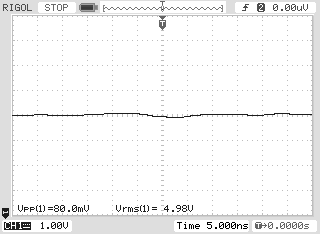
\includegraphics[width=90mm]{SM5V.png}
	\rule{35em}{0.5pt}
	\caption[Switch-mode 5V Power Supply Oscilloscope Trace]{Oscilloscope trace of the main 5V switchmode power supply showing ripple under static load.}
	\label{fig:mainpowerripple}
\end{figure}

\FloatBarrier
\subsubsection{Sensor Power Supply}

For the secondary 3.3V LDO power supply used by the board's sensor modules, an identical set of tests to those used in the verification of the main power supply were performed, using the sensor boards as the regulator output load. This yielded a ripple of 120mV, and an output voltage of 3.27V. When compared to the ADP3308 datasheet output's electrical characteristics, this was within the stated \(\pm1.2\%\) accuracy (\(3.26V\leq\text{V\subscript{out}}\leq3.34V\)).

\begin{figure}[tbph]
	\vspace{1em}
	\centering
		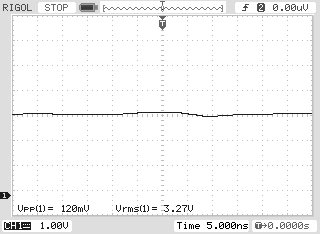
\includegraphics[width=90mm]{LDO3V.png}
	\rule{35em}{0.5pt}
	\caption[LDO 3.3V Power Supply Oscilloscope Trace]{Oscilloscope trace of the sensor 3.3V LDO power supply showing ripple under static load.}
	\label{fig:sensorpowerripple}
\end{figure}

\FloatBarrier
\subsubsection{Motor PWM Outputs}

To test the motor outputs (and, in turn, the entire motor controller circuit) the two motor output channels were connected to an oscilloscope in sequence, and a small test wrapper written over the motor driver firmware module. Each output was switched backwards and forwards at the maximum (safe) PWM rate, and the resulting waveforms verified against the expected waveforms. Figure \ref{fig:motorpwm} shows one such waveform, showing the left motor output at full speed.

\begin{figure}[tbph]
	\vspace{1em}
	\centering
		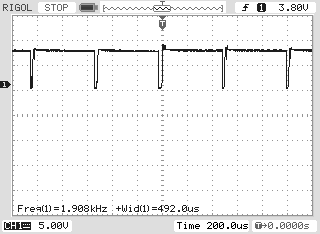
\includegraphics[width=90mm]{PWM.png}
	\rule{35em}{0.5pt}
	\caption[Motor PWM Oscilloscope Trace]{Oscilloscope trace of one motor channel PWM output while active, showing the frequency and duty cycle at full speed.}
	\label{fig:motorpwm}
\end{figure}

\FloatBarrier
\subsubsection{RGB Status LED}

A simple test routine was written to cycle through all possible colours on the mounted RGB status LED; this demonstrated that the three GPIO channels were configured and connected correctly, and that the appropriate brightness balancing for each sub-component in the LED package was set correctly by the chosen current limiting resistors on the board. As this is a simple but visually attractive piece of self-diagnostics, the test routine code was eventually retained in the final robot version during the robot's start-up sequence.

\FloatBarrier
\subsubsection{LCD and Backlight}

To test the board's LCD functions, a routine calling various formatting commands was written and wrapped around the completed LCD driver software module. These commands---containing various cursor placements, custom character definitions and formatted strings---indicated that the display was indeed working as expected. For the LCD backlight, code was written to slowly fade in the backlight brightness from the minimum value, up to the maximum in 10ms increments. Like the RGB LED test routine, this functionality was eventually incorporated into the start-up routine of the final robot firmware.

\FloatBarrier
\subsection{Software Testing}

At the conclusion of the hardware testing, a new set of software tests were performed on the robot firmware to ensure correct operation and compatibility with the appropriate specifications. This presented its own unique set of challenges, as suitable testing environments and testing procedures had to be developed.

\FloatBarrier
\subsubsection{USB Integration}

Small software tests were performed for the three supported USB classes; HID, Mass Storage and Bluetooth Adapters. Doubling as a test of the hardware drivers, the HID management driver was tested against a PS3 Controller and two generic HID class USB gaming controllers, to ensure that the appropriate buttons were mapped to the robot's functions. During these tests, a brown-out failure condition was observed on the USB bus when the robot's motors were switched on and off (or changed in direction) rapidly. This issue was traced back to the original ``AA'' cell bank battery's instantaneous current capabilities, and was temporarily corrected in the robot prototype with a large value capacitor on the battery input terminals (see Figure \ref{fig:mainpowercap}) until the more powerful Lithium-Ion battery pack was substituted.

\begin{figure}[tbph]
	\vspace{1em}
	\centering
		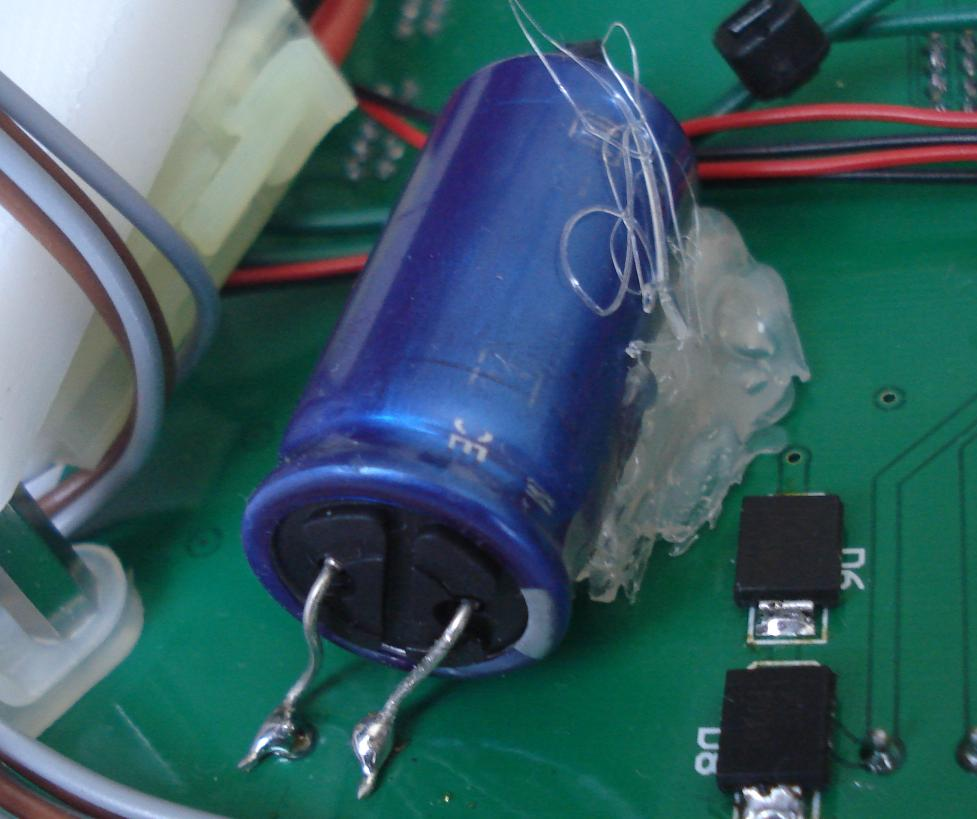
\includegraphics[width=60mm]{PowerCap.jpg}
	\rule{35em}{0.5pt}
	\caption[Temporary Main Power Input Capacitor]{Photo of the temporary main input power capacitor, to prevent brown-out conditions from motor-induced current spikes.}
	\label{fig:mainpowercap}
\end{figure}

The Mass Storage management module (and, by extension, the FATFs library it depends upon) was tested through a procedure of disk insertion and removal, with files written to and read from the disk filesystem using dummy data. Thus verified, the complete Mass Storage management file parsing routines were checked by printing the parsed file output to the robot's LCD display.

As the Bluetooth Adapter management code relied upon the upper Bluetooth Stack logical layers for correct operation, the functionality of the USB transceiver device management could not be examined and verified until the base layers on the Bluetooth Stack were completed. However, in this phase of the software testing, the module's ability to correctly bind to compatible Bluetooth devices in a generic manner (using several adapters from different manufacturers) was tested and found to function as expected.

\FloatBarrier
\subsubsection{Sensor Platform}

The sensor platform required a significant amount of time to complete and verify; the final development time was close to one and a half weeks, much more than the expected two or three days. A number of flaws were found in the written code when it was tested on the physical robot hardware, including a bug in the LUFA USB stack's I\superscript{2}C driver for packet read and writes. Timing and other issues in the written driver for the Bosch BMA150 accelerometer resulted first in no sensor output, followed by output on only one channel. The root cause of this problem was eventually tracked down to misleading datasheets, where the sensor would react correctly only if certain configuration registers were altered in specific manners to what should have been---according to the values given in the datasheet---the sensor's initial power-on defaults.

During the sensor platform testing phase additional small errors relating to the formatting and endianness of the retrieved values were also identified and corrected.

\FloatBarrier
\subsubsection{Bluetooth Stack}

The completed Bluetooth stack was tested in an iterative manner; as additional features and layers were completed, they were verified against existing third-party Bluetooth devices. An invaluable tool used in the verification and debugging of each layer and protocol was the Linux ``Bluez'' Bluetooth stack's \texttt{hcidump} tool, which allowed the robot's Bluetooth stack packets to be captured in real time and decoded, indicating any issues in the implementation of one or more protocols used in the device.

Listing \ref{lst:hcidump} shows a fragment of a HCI layer packet capture between a virtualized Linux environment and the robot, while successfully establishing a new L2CAP channel between the two devices for SDP discovery.

\lstinputlisting[float=tbph,caption={HCI packet capture during a L2CAP channel configuration.},label={lst:hcidump},language={bash}]{./Figures/HCIDump.txt}

The RFCOMM layer was examined and verified at both the L2CAP layer and the RFCOMM service layer, using the Linux \texttt{rfcomm} utility to bind the robot's virtual serial port to a virtual device node named \texttt{/dev/rfcomm0}. Connecting to this device through a standard serial terminal emulator yielded the RFCOMM layer packet dump as shown in Listing \ref{lst:rfcommdump}, showing the successful negotiation and configuration of a new RFCOMM layer multiplexer channel.

\lstinputlisting[float=tbph,caption={RFCOMM service packet capture during a multiplexer channel establishment.},label={lst:rfcommdump},language={bash}]{./Figures/RFCOMMDump.txt}

Finally, the SDP layer was verified both at the L2CAP layer packet level, and at the SDP layer using the Linux tool \texttt{sdptool}. This utility was used to browse the services offered from the robot's SDP server service, to ensure that the correct services and service attributes were being sent to the requesting device correctly. A sample of this SDP output is shown in Listing \ref{lst:sdpbrowse}.

\lstinputlisting[float=tbph,caption={Capture of the services and attributes exposed by the robot's SDP server.},label={lst:sdpbrowse},language={bash}]{./Figures/SDPBrowse.txt}

\section{Achieved Results}

At the conclusion of the project time frame, much of the project goals had been achieved. The completed robot hardware was demonstrated as working with a variety of off-the-shelf consumer grade Bluetooth products, including the Playstation 3 controller, Nintendo Wii controller and a Sony Ericsson z550i mobile phone running its included \textit{Bluetooth Remote Control} application (see Figure \ref{fig:workingbtcontrollers}). The Bluetooth stack developed for the project was found to be functional enough to operate with these devices without special modifications being required to either the robot or the Bluetooth controllers.

\begin{figure}[tbph]
	\vspace{1em}
	\centering
		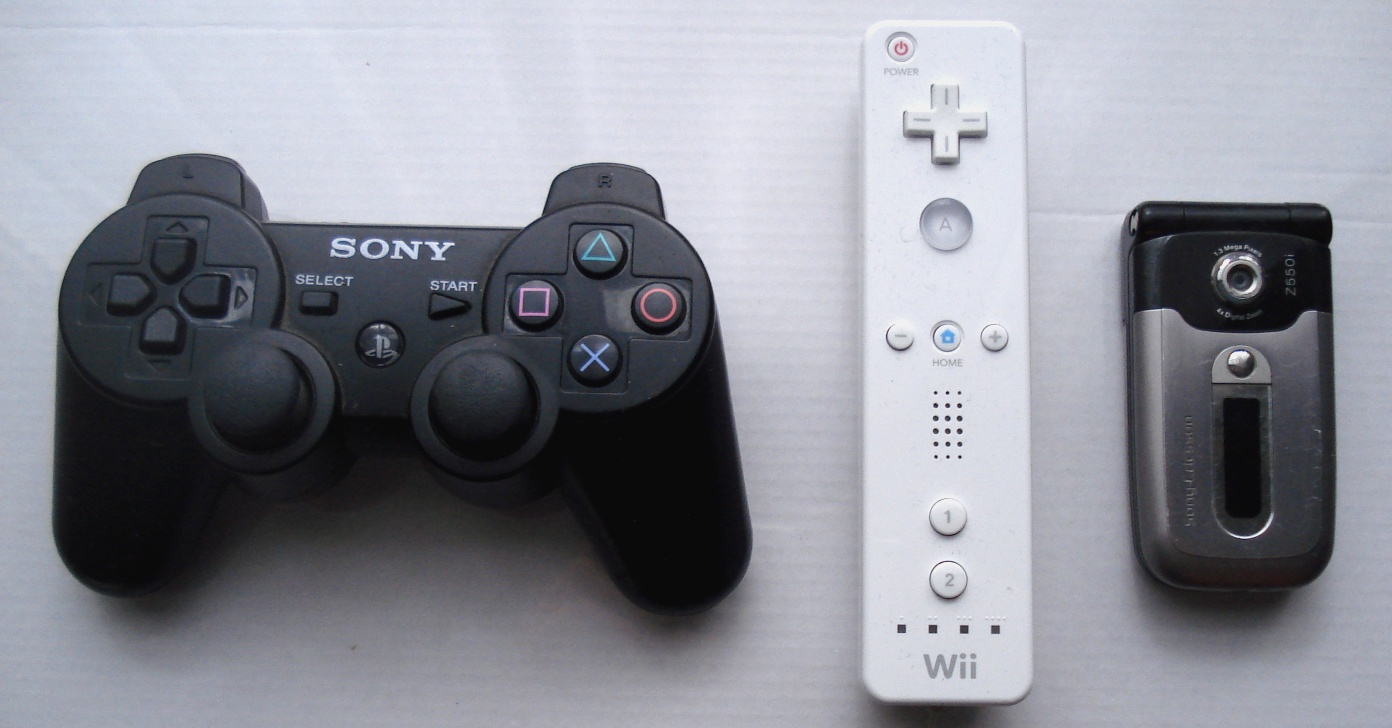
\includegraphics[width=140mm]{BluetoothControllers.jpg}
	\rule{35em}{0.5pt}
	\caption[Tested Working Controllers]{Tested consumer grade Bluetooth enabled devices: \\ Playstation 3 controller \textit{(left)}, Nintendo Wii controller \textit{(middle)}, Sony-Ericsson z550i mobile phone \textit{(right)} }
	\label{fig:workingbtcontrollers}
\end{figure}

All the robot's sensors and other hardware drivers worked correctly, with the user able to control the robot's movement, headlights and horn over both wired USB and wireless Bluetooth HID connections. Sensor data was able to be streamed remotely to a PC or other Bluetooth enabled device supporting the RFCOMM wireless serial port profile. Listing \ref{lst:sensorstream} shows a sample of the streaming sensor data captured from the robot.

\lstinputlisting[float=tbph,caption={Captured RFCOMM streaming sensor data.},label={lst:sensorstream},language={bash}]{./Figures/SensorStream.txt}

A simple C\# application was written to display the streaming sensor data graphically to the user in real time (see Figure \ref{fig:sensorhostapp}). The robot firmware was capable of maintaining both the streaming sensor data connection as well as a secondary connection to a Bluetooth controller simultaneously, allowing for user control of the robot while a PC graphs the retrieved sensor values.

\begin{figure}[tbph]
	\vspace{1em}
	\centering
		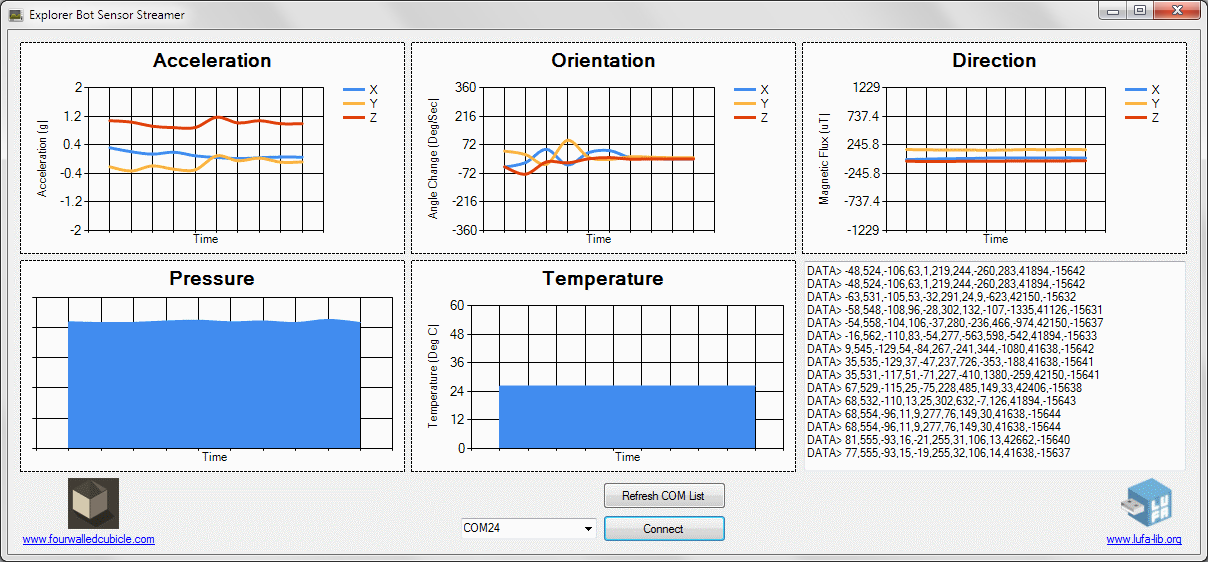
\includegraphics[width=140mm]{SensorDataApp.png}
	\rule{35em}{0.5pt}
	\caption[Sensor Logging Host Application]{Sensor logging application, showing data streaming wirelessly from the connected robot via a Bluetooth virtual serial port. }
	\label{fig:sensorhostapp}
\end{figure}

The completed robot PCB hardware was integrated into a pre-fabricated off-the-shelf robot platform base, and linked to the two wheel mounted DC motors. Additional parts for the PCB retention clip and headlight and horn mounting were designed by the project's Co-Supervisor Robert Ross, and printed out on the University's 3D printer. This resulted in the compact and functional robot prototype shown in Figure \ref{fig:completedrobot}.

\begin{figure}[tbph]
	\vspace{1em}
	\centering
		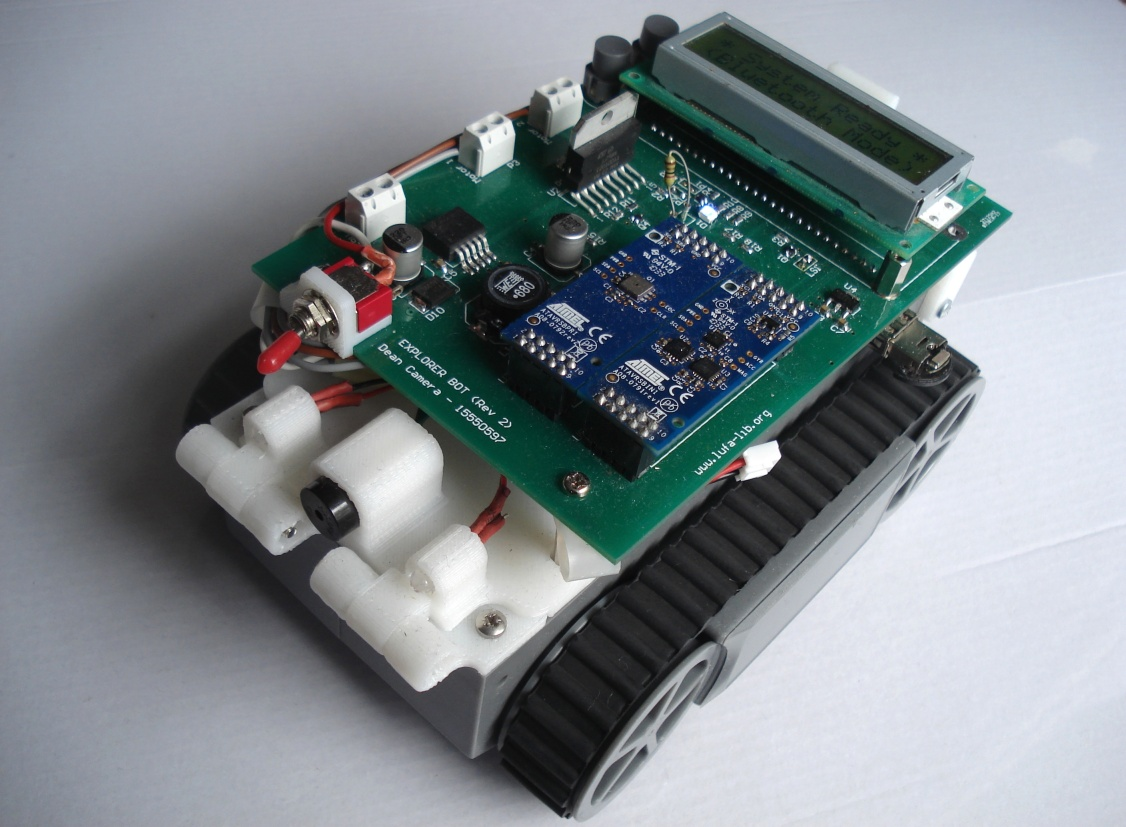
\includegraphics[width=140mm]{CompletedRobot.jpg}
	\rule{35em}{0.5pt}
	\caption[Photo of Completed Robot]{Photo of the completed \textit{ExplorerBot} prototype robot}
	\label{fig:completedrobot}
\end{figure}
